% датасет
% * smt-comp
% * usvm
% * метрики
% roberta
% gnn
% результаты

% todo: ещё куда-нибудь обязательно надо вхуячить ссылку на ksmt

% todo: написать про то, как работает message passing neural network
% todo:
% * квантизация
% * аугментации
% * кванторные формулы

\section{Датасет}

В своей работе я использовал два датасета с SMT-формулами:

\begin{enumerate}
    \item Бенчмарк\footnote{Набор данных для тестирования корректности или производительности программы.} с SMT-COMP 2023 \cite{smt-comp-2023-benchmarks}.
    \item Формулы, собранные в процессе работы символьного движка USVM.
\end{enumerate}

% todo: здесь ссылка на USVM (Поспелов, 2023)

\subsection{SMT-COMP}

В процессе исследований этот бенчмарк был поделен на три части:

\begin{enumerate}
    \item \texttt{BitVec} --- формулы из логики \texttt{QF\_BV}, обычные формулы с битовыми векторами;
    \item \texttt{SymbEx} --- формулы из логик \texttt{QF\_BV}, \texttt{QF\_ABV}, \texttt{QF\_ABVFP}, \texttt{QF\_AUFBV}, \\ \texttt{QF\_AUFBVFP}, \texttt{QF\_BVFP}, \texttt{QF\_FP}, \texttt{QF\_UF}, \texttt{QF\_UFBV} и \texttt{QF\_UFFP}, которые возникают в процессе работы любого движка для символьного исполнения;
    \item \texttt{QuaFree} --- формулы из всех безкванторных логик, включая \texttt{QF\_LIA}, \texttt{QF\_NRA}, \texttt{QF\_BVFPLRA} и т. д..
\end{enumerate}

Такое разделение обусловлено тем, что для анализа качества хочется смотреть, как модель обучается и какое качество она выдаёт на формулах из разных логик. Однако, к сожалению, большинство логик в данном бенчмарке содержат слишком мало данных, чтобы можно было провести анализ на них, поэтому было принято решение объединить логики в группы по смыслу. Логика \texttt{QF\_BV} была вынесена в отдельную группу, поскольку она является самой многочисленной, а также самой важной на практике. Логики из группы \texttt{SymbEx} были собраны вместе, поскольку моя текущая задача существует в контексте символьного исполнения, поэтому хочется отдельно анализировать способность модели решать подобные формулы. В оставшуюся группу \texttt{QuaFree} попали все безкванторные логики, т. к. хочется также анализировать способность модели решать задачу в некотором общем случае. В дальнейшем каждую группу будем называть датасетом с соответствующим именем.

Формулы с кванторами в данной работе не рассматривались вообще, т. к. они существенно сложнее безкванторных, и их было решено отложить до лучших времён.

Чтобы данные влезли на видеокарту в каждом датасете были оставлены только формулы размером\footnote{Размером формулы считаем количество переменных, констант и операций в ней. Например, размер формулы $(x + y = 5) \vee (z = 3)$ равен 9.} не более 10\,000 и глубиной\footnote{Глубиной формулы считаем максимальную вложенность переменных, констант и операций в ней. Например, глубина формулы $(x + y = 5) \vee (z = 3)$ равна 4.} не более 2\,000. Итоговые параметры построенных датасетов отображены в таблице~\ref{smt-comp-datasets-table}.

\begin{table}[ht]
\begin{center}
\begin{tabular}{r|cccc}
    Датасет & \makecell{Количество \\ формул} & \makecell{Средний \\ размер \\ формулы} & \makecell{Средняя \\ глубина \\ формулы} & \makecell{Доля \\ выполнимых \\ формул} \\
    \hline \hline
    \rule{0pt}{2.5ex}
    \texttt{BitVec} & 33\,797 & 1181.92 & 85.45 & 0.378 \\
    \texttt{SymbEx} & 85\,078 & 669.46 & 49.24 & 0.611 \\
    \texttt{QuaFree} & 123\,396 & 965.16 & 48.71 & 0.622 \\
\end{tabular}
\caption{\label{smt-comp-datasets-table} Параметры датасетов, полученных из данных с SMT-COMP 2023 \cite{smt-comp-2023-benchmarks}.}
\end{center}
\end{table}

\subsection{USVM}

% todo: здесь тоже ссылка на USVM (Поспелов, 2023)

Для проверки возможности применения модели на практике были также вручную собраны датасеты, состоящие из формул, которые возникают в процессе работы символьного движка USVM. Сбор осуществлялся с помощью простого логирования формул, на которых вызывался SMT-решатель. Разные датасеты получались при запуске движка на разных проектах или наборах программ. Подобным образом были собраны три тренировочных и восемнадцать валидационных датасетов.

Такое строгое разделение на тренировочные и валидационные датасеты вдобавок к такому большому количеству вторых обусловлено желанием проверить обобщающую способность модели: хочется, чтобы модель показывала хорошее качество на формулах, возникающих при запуске движка на любых программах; при этом, нет никаких гарантий, что при переходе от одного набора программ к другому распределение, из которого порождаются формулы, изменится несущественно, и качество модели, обученной на данных из другого распределения, упадёт не слишком сильно.

Тренировочные датасеты были собраны на следующих программах:

\begin{enumerate}
    \item \texttt{usvm-test} --- на наборе программ для unit и интеграционного тестирования USVM;
    \item \texttt{the-algorithms} --- на репозитории с реализациями различных теоретических и практических алгоритмов на Java;
    \item \texttt{usvm-core} --- на ядре символьного движка USVM (движок был запущен на самом себе).
\end{enumerate}

Параметры тренировочных датасетов указаны в таблице~\ref{usvm-train-datasets-table}.

\begin{table}[ht]
\begin{center}
\begin{tabular}{r|cccc}
    Датасет & \makecell{Количество \\ формул} & \makecell{Средний \\ размер \\ формулы} & \makecell{Средняя \\ глубина \\ формулы} & \makecell{Доля \\ выполнимых \\ формул} \\
    \hline \hline
    \rule{0pt}{2.5ex}
    \texttt{usvm-test} & 153\,778 & 522.84 & 5.18 & 0.038 \\
    \texttt{the-algorithms} & 181\,633 & 277.03 & 23.94 & 0.066 \\
    \texttt{usvm-core} & 192\,744 & 179.42 & 12.19 & 0.066 \\
\end{tabular}
\caption{\label{usvm-train-datasets-table} Параметры тренировочных датасетов, собранных в процессе работы USVM.}
\end{center}
\end{table}

Валидационные датасеты были собраны при запуске USVM на следующих проектах, написанных на Java и других JVM-языках:

\begin{enumerate}
    \item \texttt{owasp} --- OWASP\footnote{Open Web Application Security Project.}, открытый бенчмарк из программ на Java, на котором оценивают качество инструментов для автоматического поиска уязвимостей в коде \cite{owasp-website};
    \item \texttt{cassandra} --- Apache Cassandra, распределённая NoSQL СУБД\footnote{Система Управления Базами Данных.} \cite{cassandra-website};
    \item \texttt{kafka} --- Apache Kafka, распределённый брокер сообщений \cite{kafka-website};
    \item \texttt{spark-core} --- Apache Spark, система для распределённой обработки данных (модуль ядра) \cite{spark-website};
    \item \texttt{spark-streaming} --- тот же Spark (модуль потоковой обработки данных);
    \item \texttt{utbot-core} --- UnitTestBot, инструмент для автоматической генерации unit-тестов (модуль ядра) \cite{utbot-github};
    \item \texttt{utbot-java} --- тот же UnitTestBot (модуль генерации тестов для Java);
    \item \texttt{utbot-python} --- тот же UnitTestBot (модуль генерации тестов для Python);
    \item \texttt{utbot-js} --- тот же UnitTestBot (модуль генерации тестов для языка JavaScript);
    \item \texttt{utbot-go} --- тот же UnitTestBot (модуль генерации тестов для Go);
    \item \texttt{zookeeper} --- Apache Zookeeper, служба для координации распределённых систем \cite{zookeeper-website};
    \item \texttt{elasticsearch} --- Elasticsearch, встраиваимая система для текстового поиска \cite{elasticsearch-website};
    \item \texttt{hbase} --- Apache HBase, распределённая табличная база данных \cite{hbase-website};
    \item \texttt{guava} --- Google Guava, набор библиотек-расширений для Java \cite{guava-website};
    \item \texttt{hadoop-common} --- Apache Hadoop, экосистема для распределённого хранения и обработки данных (модуль ядра) \cite{hadoop-website};
    \item \texttt{hadoop-hdfs} --- тот же Hadoop (модуль распределённой файловой системы);
    \item \texttt{hadoop-mapreduce} --- тот же Hadoop (модуль для распределённых вычислений в парадигме MapReduce);
    \item \texttt{hadoop-yarn} --- тот же Hadoop (модуль планировщика ресурсов);
\end{enumerate}

Параметры валидационных датасетов указаны в таблице~\ref{usvm-val-datasets-table}.

\begin{table}[ht]
\begin{center}
\begin{tabular}{r|cccc}
    Датасет & \makecell{Количество \\ формул} & \makecell{Средний \\ размер \\ формулы} & \makecell{Средняя \\ глубина \\ формулы} & \makecell{Доля \\ выполнимых \\ формул} \\
    \hline \hline
    \rule{0pt}{2.5ex}
    \texttt{owasp} & 30\,935 & 3169.44 & 27.0 & 0.029 \\
    \texttt{cassandra} & 13\,896 & 164.84 & 11.73 & 0.057 \\
    \texttt{kafka} & 46\,867 & 5103.27 & 18.93 & 0.083 \\
    \texttt{spark-core} & 14\,504 & 5599.33 & 28.0 & 0.061 \\
    \texttt{spark-streaming} & 69\,254 & 1168.64 & 8.31 & 0.057 \\
    \texttt{utbot-core} & 31\,043 & 4570.6 & 28.95 & 0.061 \\
    \texttt{utbot-java} & 12\,492 & 116.4 & 10.71 & 0.045 \\
    \texttt{utbot-python} & 24\,893 & 266.66 & 6.04 & 0.115 \\
    \texttt{utbot-js} & 13\,276 & 2286.54 & 133.8 & 0.062 \\
    \texttt{utbot-go} & 43\,988 & 281.69 & 19.21 & 0.014 \\
    \texttt{zookeeper} & 38\,631 & 1196.51 & 47.23 & 0.046 \\
    \texttt{elasticsearch} & 38\,967 & 388.62 & 19.72 & 0.001 \\
    \texttt{hbase} & 38\,049 & 3513.78 & 90.81 & 0.019 \\
    \texttt{guava} & 56\,607 & 545.98 & 34.99 & 0.014 \\
    \texttt{hadoop-common} & 41\,255 & 419.05 & 10.32 & 0.081 \\
    \texttt{hadoop-hdfs} & 109\,294 & 2795.7 & 210.87 & 0.032 \\
    \texttt{hadoop-mapreduce} & 12\,044 & 1294.2 & 47.17 & 0.011 \\
    \texttt{hadoop-yarn} & 32\,555 & 120.71 & 13.01 & 0.035 \\
\end{tabular}
\caption{\label{usvm-val-datasets-table} Параметры валидационных датасетов, собранных в процессе работы USVM.}
\end{center}
\end{table}

Отмечу, что в валидационных датасетах также отобраны формулы, размер и глубина которых не превышает 10\,000 и 2\,000 соответственно, но, помимо этого, здесь добавилось ещё одно условие: размер должен быть не меньше некоторого значения, которое подбиралось эмпирическим путём отдельно для каждого датасета (и которое можно угадать, если посмотреть на средний столбец в таблице). Поэтому формулы из валидационных датасетов кажутся больше, чем из тренировочных. Это было сделано, чтобы уменьшить объём данных и ускорить вычисления, а также чтобы оценивать качество модели именно на больших формулах, т. к. кажется, что на практике модель должна существенно помогать движку именно в этом случае.

Ещё внимательный читатель может заметить, что во всех датасетах из формул, собранных в процессе работы USVM, есть огромный дисбаланс классов: меньше десяти процентов формул являются выполнимыми. На самом деле, в этом нет ничего неожиданного, потому что в процессе символьного исполнения программы SMT-решателю действительно чаще всего приходится иметь дело с невыполнимыми формулами.

% todo: кажется, тут стоит ещё дописать
% todo: и ещё можно заменить таблицы на ящики с усами

\subsection{Метрики}

% todo: дописать, почему нам нужны такие метрики

% todo: текстовый подход
% \section{Текстовый подход}

\section{Подход с использованием GNN}

\subsection{Устройство GNN} \label{gnn-architecture}

Графовые нейронные сети, наряду со свёрточными, рекуррентными и т. д., являются одним из способов решать задачу машинного обучения, учитывая специфику данных. Так как графы отображают взаимоотношения между объектами некоторого множества, то и процесс построения модели, в данном случае, учитывает локальность и связи между произвольными объектами из предметной области.

Впервые архитектура GNN в общем виде была описана ещё в 2009 году в статье \cite{gnn-intro-paper}, однако широкую известность получила только в 2017 году после её применения для предсказания квантовых чисел в вычислительной органической химии \cite{gnn-quantum-chemistry-paper}. В основе вычислений лежит процесс \textit{передачи сообщений} между вершинами графа, который изображён на рис.~\ref{message-passing-nn-architecture}: в каждой вершине хранится вектор-состояние (эмбеддинг), и на каждом шаге все вершины сначала рассылают свой текущий вектор всем своим непосредственным соседям, а потом агрегируют пришедшие от соседей векторы (\textit{сообщения}) и обновляют свой вектор-состояние с учётом этого; далее эти шаги повторяются несколько раз, после чего полученные таким образом векторы-состояния используются для построения представления графа и дальнейшего решения задачи.

\begin{figure}[ht]
\begin{center}
    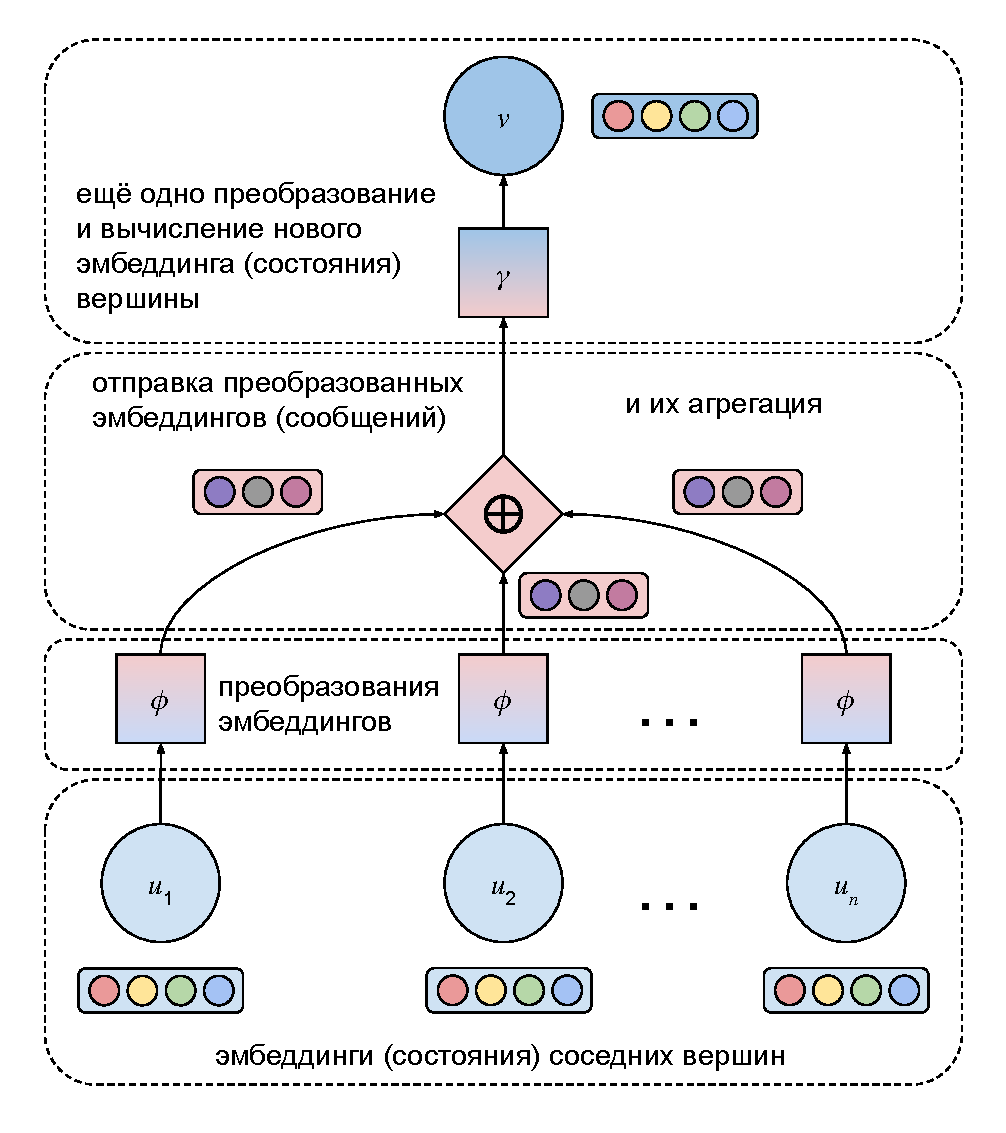
\includegraphics[scale=0.75]{./assets/message-passing-nn-architecture.pdf}
    \caption{\label{message-passing-nn-architecture} Схема обновления вектора-состояния вершины $v$ через векторы-сообщения от её соседей $u_1$, $u_2$, \ldots, $u_n$. Цвет (синий / красный) обозначает размерность. Более тёмный цвет вверху обозначает обновлённое состояние.}
\end{center}
\end{figure}

Формально весь процесс устроен следующим образом:

\begin{itemize}
    \item у каждого ребра $e$ есть набор параметров $s_e \in \mathbb{R}^m$;
    \item в начале вычислений в каждой вершине $v$ содержится содержится вектор (состояние) $x_v^{(0)} \in \mathbb{R}^n$ с некоторой информацией;
    \item производится несколько итераций \textit{передачи сообщений}, на $t$-й из них производится обновление векторов в вершинах по правилу, которое описывается формулой~(\ref{gnn-state-update-rule});
    \item после всех итераций предполагается, что вычисленные векторы (состояния) образуют некоторое представление вершины / графа, поэтому их можно использовать в качестве признаков вершины / графа, подавая в какую-нибудь MLP-сеть.
\end{itemize}

\begin{equation} \label{gnn-state-update-rule}
    x_v^{(t)} = \gamma^{(t)} \left(x_v^{(t - 1)}, \bigoplus_{u \in \mathcal{N}(v)} \phi^{(t)} \left(x_v^{(t - 1)}, x_u^{(t - 1)}, s_{e(u \, \to \, v)} \right) \right)
\end{equation}

Обозначения в формуле~(\ref{gnn-state-update-rule}):

\begin{itemize}
    \item $x_v^{(t)} \in \mathbb{R}^n$ --- описанные выше эмбеддинги вершин;
    \item $e(u \, \to \, v)$ --- ребро из вершины $u$ в вершину $v$, а $s_{e(u \, \to \, v)} \in \mathbb{R}^m$ --- его параметры;
    \item $\mathcal{N}(v)$ --- окрестность вершины $v$;
    \item $\phi^{(t)}: \mathbb{R}^n \times \mathbb{R}^n \times \mathbb{R}^m \to \mathbb{R}^k$ --- функция создания сообщения по состояниям вершин и параметрам ребра; может быть представлена аффинным преобразованием, композицией линейных слоёв и нелинейных активаций или просто любым дифференцируемым преобразованием с обучаемыми или необучаемыми параметрами;
    \item $\bigoplus: \mathbb{R}^k \to \mathbb{R}^k$ --- функция агрегации, например: сумма, среднее или взвешенная сумма с учётом механизма внимания;
    \item $\gamma^{(t)}: \mathbb{R}^n \times \mathbb{R}^k \to \mathbb{R}^n$ --- функция обновления вектора-состояния (эмбеддинга) вершины; аналогична $\phi^{(t)}$.
\end{itemize}

В качестве примера построения сети по такой схеме можно рассмотреть Graph Convolutional Network \cite{gcn-conv-paper}, самую популярную GNN-архитектуру. В её случае мы имеем:

\begin{itemize}
    \item $\phi^{(t)} = W^T \cdot x_u^{(t - 1)}$;
    \item $\bigoplus = \sum \limits_{u \in \mathcal{N}(v) \cup \{v\}} \dfrac{1}{\sqrt{|\mathcal{N}(v)|} \cdot \sqrt{|\mathcal{N}(u)|}} \cdot \phi^{(t)} \left(x_v^{(t - 1)}, x_u^{(t - 1)}, s_{e(u \, \to \, v)} \right)$;
    \item $\gamma^{(t)} = \bigoplus \limits_{u \in \mathcal{N}(v)} \phi^{(t)} \left(x_v^{(t - 1)}, x_u^{(t - 1)}, s_{e(u \, \to \, v)} \right) + b$;
\end{itemize}

\noindent где матрица весов $W$ и вектор-сдвиг $b$ являются выучиваемыми параметрами. Итого получаем:

\begin{equation}
    x_v^{(t)} = \sum \limits_{u \in \mathcal{N}(v) \cup \{v\}} \dfrac{1}{\sqrt{|\mathcal{N}(v)|} \cdot \sqrt{|\mathcal{N}(u)|}} \cdot \left(W^T \cdot x_u^{(t - 1)} \right) + b
\end{equation}

В настоящий момент GNN широко применяются для решения задач вычислительной физики, химии и биологии, построения рекомендательных систем, прогнозирования трафика на дорогах, распознавания объектов, синтеза текстов и речи \cite{gnn-global-overview} \cite{gnn-deep-learning-5g}.

\subsection{Архитектура нейронной сети для решения задачи}

% formula ast
% * vars and consts

% RvNN

% sage conv
% transformer conv

\section{Эксперименты и результаты}

% todo: тут в основной части можно красивый барплот, а в приложении огромную таблицу
